\documentclass[]{report}
\usepackage{listings}
\usepackage[margin=1.25in]{geometry}
\usepackage{graphicx}


% Title Page
\title{Comparing the Performance of Implicit and Explicit Concurrency in Java}
\author{Dominic Rathbone}


\begin{document}
\maketitle

\section*{Introduction}
In order to compare the effects of concurrency in Java on performance, A test program was created that compared various implementations of concurrency, implicit and explicit, to a baseline non-concurrent implementation. These implementations performed a mathematical operation finding all the mersenne primes in a set on a set of integers derived from the user inputting a start and end number at launch. Time (in nano seconds) was used as a benchmark in order to compare these implementations. The time was taken before and after each implementation ran over the set and then the total run time was derived from them. In order to compare them with ease, a ratio derived from dividing the total time of the baseline implementation by the total time of concurrent implementation is outputted to csv files. To run the programs, I am using a ThinkPad laptop running Fedora with a quad-core 2.50GHz i5-2520M CPU and 8 gigabytes of RAM. as well as a Gaming PC running Windows 7 with a quad-core 3.50GHz i5 4690K and 8 gigabytes of RAM.

\section{Non-concurrent Approach}
The non-concurrent approach runs the operations sequentially, running over the sequence of integers with a for statement and incrementing a counter every time a prime number is found. This is used as the baseline to compare the implicit and explicit concurrent approaches to.(see Appendix A)

\section{Multi-threading}
The first explicitly concurrent implementation uses raw threads to run the operations over the sequence of numbers. This was attempted in two ways. First of all, to make the test fairer, I produced an implementation that spawned a new thread for every number in the sequence (see Appendix B, figure 1), similar to how a parallel stream would split a stream of numbers into multiple parallel sub-streams. On testing this implementation, it was revealed that this would not be an efficient way to approach concurrency because  as the sequence of numbers became larger, it would become extremely slow. This was due to the lack of thread management such as a queue or limit to how many threads should be started at once meaning the machine was being flooded with threads. As a result of this, the implementation was revised and it was decided that the best way to approach this was to split the sequence of numbers down into smaller sequences using the number of cores with one thread for each sequence (see Appendix B, figure 2). This would mean that although each CPU core had to process with a larger sequence of numbers per thread, the number of threads and the overhead associated with them was lower which meant the time was significantly faster.
 
\section{Thread Pooling}
The second explicitly concurrent implementation was through the use of thread pools and futures. The thread pool is a group of pre-defined threads that can be used to run tasks. In this approach, a task is submitted to the thread pool for every number in the sequence. This is similar to the raw multi-threaded implementation but the thread pool can queue the threads so they do not start at the same time, bottlenecking the machine. The results of this task is then retrieved through the future object that results from the submission of the task. (see Appendix C).

\section{Streaming}
This is how implicit concurrency can be achieved in Java 8. It takes the sequence of number, processing it as a stream and applying intermediate operations on each element in this stream until it reaches an aggregate (terminal) operation which ends the set of operations. This can be done sequentially with a serial stream (see Appendix D) or concurrently with a parallel stream.(see Appendix E)

\section{Data Analysis}

\appendix
\chapter{}
\begin{figure}[h!]
	\caption{Non-concurrent}
	\begin{lstlisting}[language=Java,frame=single]
public static void nonConcurrent() {
	for ( long n = START; n < END; n++ ) {
		int primeCount = 0;
		if (Calculator.isMersennePrime(n)) {
			primeCount++;
		}
	}
}
	\end{lstlisting}
\end{figure}

\chapter{}
\begin{figure}[h!]
	\caption{Multi-threaded 1}
	\begin{lstlisting}[language=Java,frame=single]
public static void multiThreaded() {
	List<Thread> threads = new ArrayList<>();
		for (long n = START; n < END; n++) {
			Thread thread = new Thread(
				new RunnableA(n)
			);
			thread.start();
			threads.add(thread);
		}
		for(Thread thread: threads) {
			try {
				thread.join();
			} catch (InterruptedException e){
				e.printStackTrace();
			}
		}
}
	\end{lstlisting}
\end{figure}

\begin{figure}[h!]
	\caption{Multi-threaded 2}
	\begin{lstlisting}[language=Java,frame=single]
public static void multiThreaded2() {

	List<Thread> threads = new ArrayList<>();
	long subsequence = (END - START) / CORES;
	
	for ( long n = START; n < END; n=n+subsequence) {
		Thread thread = new Thread(
			new RunnableB(n, n+subsequence)
		);
		thread.start();
		threads.add(thread);
	}
	
	for(Thread thread: threads) {
		try {
			thread.join();
		} catch (InterruptedException e) {
			e.printStackTrace();
		}
	}
}
	\end{lstlisting}
\end{figure}

\chapter{}
\begin{figure}[h!]
	\caption{Thread Pool}
	\begin{lstlisting}[language=Java,frame=single]
public static void threadPool() {
	ExecutorService executorService =
		Executors.newFixedThreadPool(CORES);
	ArrayList<Future<Integer>> futures =
		new ArrayList<>();
	
	for ( long n = START; n < END; n++ ) {
		final long number = n;
		Future<Integer> future =
		executorService.submit(() -> {
		  if(Calculator.isMersennePrime(number)) {
			  return 1; 
		  }
		  else {
			  return 0;
		  }
		}
		);
		futures.add(future);
	}
	
	int primeCount = 0;
	for (Future<Integer> future : futures) {
		try {
			primeCount += future.get();
		} catch (Exception e) {
		}
	}
	executorService.shutdown();
}
	\end{lstlisting}
\end{figure}

\chapter{}
\begin{figure}[h!]
	\caption{Serial Stream}
	\begin{lstlisting}[language=Java,frame=single]
public static void serialStream() {
	long primeCount = Stream
	.iterate(START, n -> n + 1)
	.limit(END-START)
	.filter( n -> Calculator.isMersennePrime(n) )
	.count();
}
	\end{lstlisting}
\end{figure}
\chapter{}
\begin{figure}[h!]
	\caption{Parallel Stream}
	\begin{lstlisting}[language=Java,frame=single]
public static void parallelStream() {
	long primeCount = Stream
	.iterate(START, n -> n + 1)
	.limit(END-START)
	.parallel()
	.filter(n -> Calculator.isMersennePrime(n) )
	.count();
}
	\end{lstlisting}
\end{figure}

\chapter{}
\begin{figure}[h!]
	\caption{PC Results}
	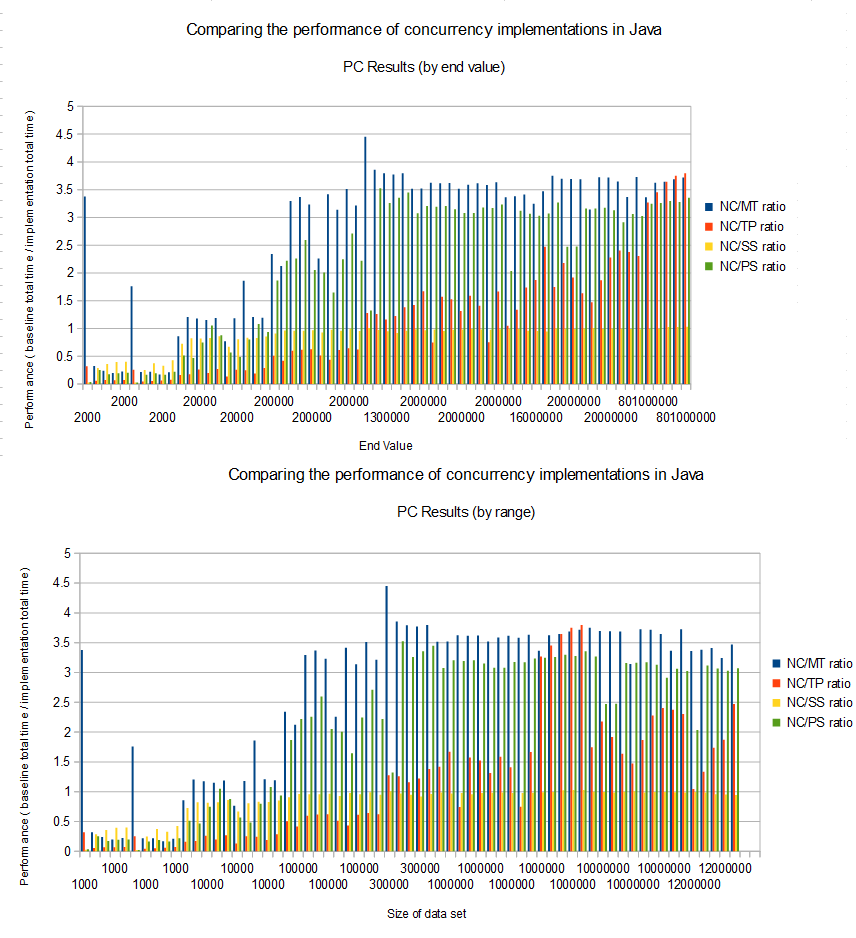
\includegraphics[scale=0.75]{PC_GRAPHS.png}
\end{figure}

\chapter{}
\begin{figure}[h!]
	\caption{Laptop Results}
	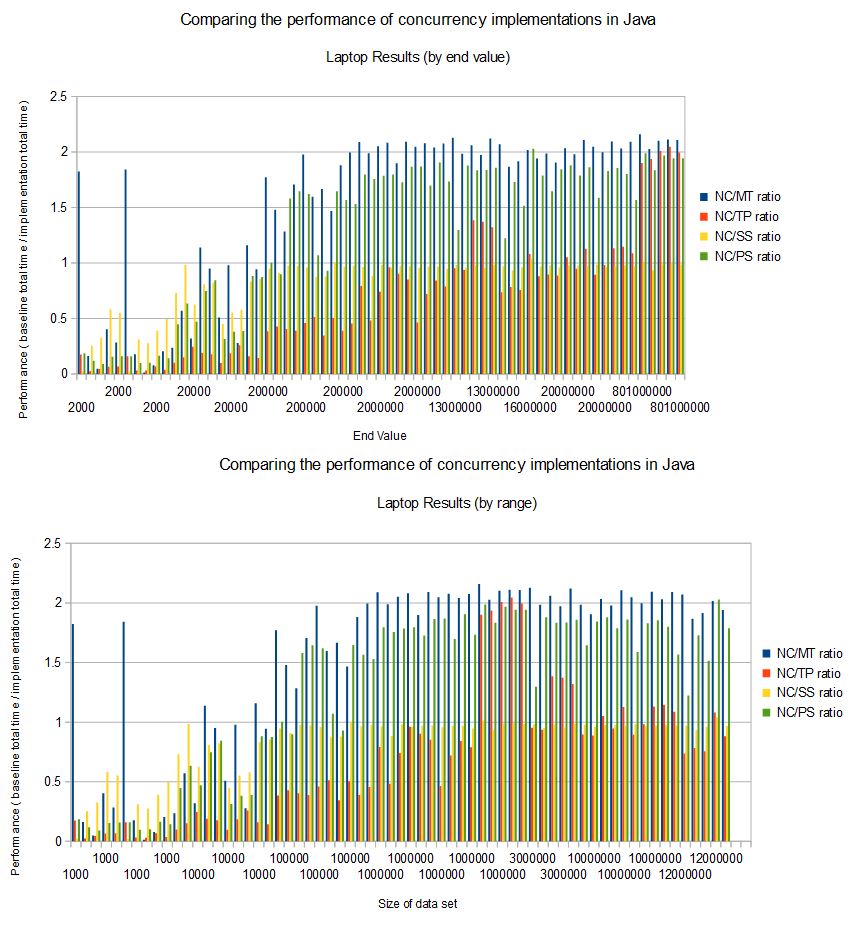
\includegraphics[scale=0.75]{LAPTOP_GRAPHS.png}
\end{figure}
\end{document}          
